\section{Mediciones}

\subsection{Instrumental utilizado}

Para las mediciones se utilizó un osciloscopio \textit{Tektronix MSO 70404C},
en la figura \ref{fig:osciloscopio} puede observarse el mismo. El instrumento 
posee \qty{4}{\giga\hertz} de ancho de banda analógico, y una tasa de muestreo
de \qty[per-mode=symbol]{25}{\giga\siemens\per\second} \cite{oscilloscope_datasheet}.

\subsubsection{Seguridad del instrumento}

La impedancia de entrada de entrada del instrumento es de \qty{50}{\ohm} y cumplía 
el rol de carga para el generador de pulsos. Dado el cuantioso costo del
instrumento, era fundamental garantizar que el circuito bajo ninguna condición
fuera a entregar una potencia potencialmente peligrosa para el mismo.

El osciloscopio tiene especificada una tensión de entrada máxima de $5 \ V_{RMS}$
para una resolución $\geq \ 100 \ mV/div$ y $1 \ V_{RMS}$ para una resolución
$< \ 100 \ mV/div$.

En condiciones normales de funcionamiento, la potencia disipada por la carga es
mínima, ya que es la potencia que disipa el tren de pulsos en un carga de
\qty{50}{\ohm}. \textcolor{red}{REFERENCIAR ACÁ LA SECCIÓN DONDE SE DESARROLLA
ESTA EXPRESIÓN}.

No solo es necesario analizar la disipación de potencia en condiciones normales
de funcionamiento, sino también para el caso de una falla, ya que el principal
objetivo es garantizar la integridad del instrumento en cualquier condición.

En caso de haber alguna falla con algún componente del circuito, el \textit{stub}
de salida provee una función de protección. Este componente, para señales con
una variación temporal mucho mayor al largo del mismo, actúa como una puesta a
tierra.

Entonces, la componente de continua a la salida del generador de pulsos tiene un
valor esperado de \qty{0}{\volt}, tanto para condiciones normales de 
funcionamiento como en presencia de fallas.

En cuanto a la componente alterna de la salida, su valor esperado es
extremadamente bajo, ya que únicamente señales de gran ancho de banda pueden ser
filtradas y permanecer con una amplitud considerable a la salida del 
\textit{stub}.

\begin{figure}
  \centering
    \includegraphics[width=0.6\textwidth]{images/osciloscopio.png}
    \caption{Osciloscopio XXXX}
    \label{fig:osciloscopio}
\end{figure}

\subsection{Banco de medición}

En la figura \ref{fig:banco_medicion} puede observarse el esquema del banco de
medición. Consistió de

\begin{itemize}
    \item{Placa FPGA: consistía de una FPGA XXXX. Esta generaba el pulso
        cuadrado de control del driver. Este componente determina el ciclo de
        trabajo.}
    \item{Fuente de alimentación: provee DC para el driver. La amplitud de esta
        fuente determina la amplitud del pulso unipolar del driver.}
    \item{Driver: tiene tres funciones: actuar como buffer para la FPGA, de
        manera que la carga exigida sea baja, convertir la amplitud digital del
        pulso de la FPGA a la amplitud de la fuente de alimentación, y convertir
        el pulso unipolar en uno bipolar.}
\end{itemize}

\subsubsection{Fuente de alimentación}

La fuente de alimentación era una XXXXX, en la figura \ref{fig:mediciones_fuente}. Permitía generar amplitudes de entre
XXX y XXX y tenía una máxima capacidad de corriente de XXXXX.

Presentaba limitación de corriente regulable e indicadores para la amplitud y la
corriente entregada, lo que permitía trabajar de manera segura, dentro de los
límites de consumo obtenidos en las simulaciones anteriores.

\begin{figure}
  \centering
    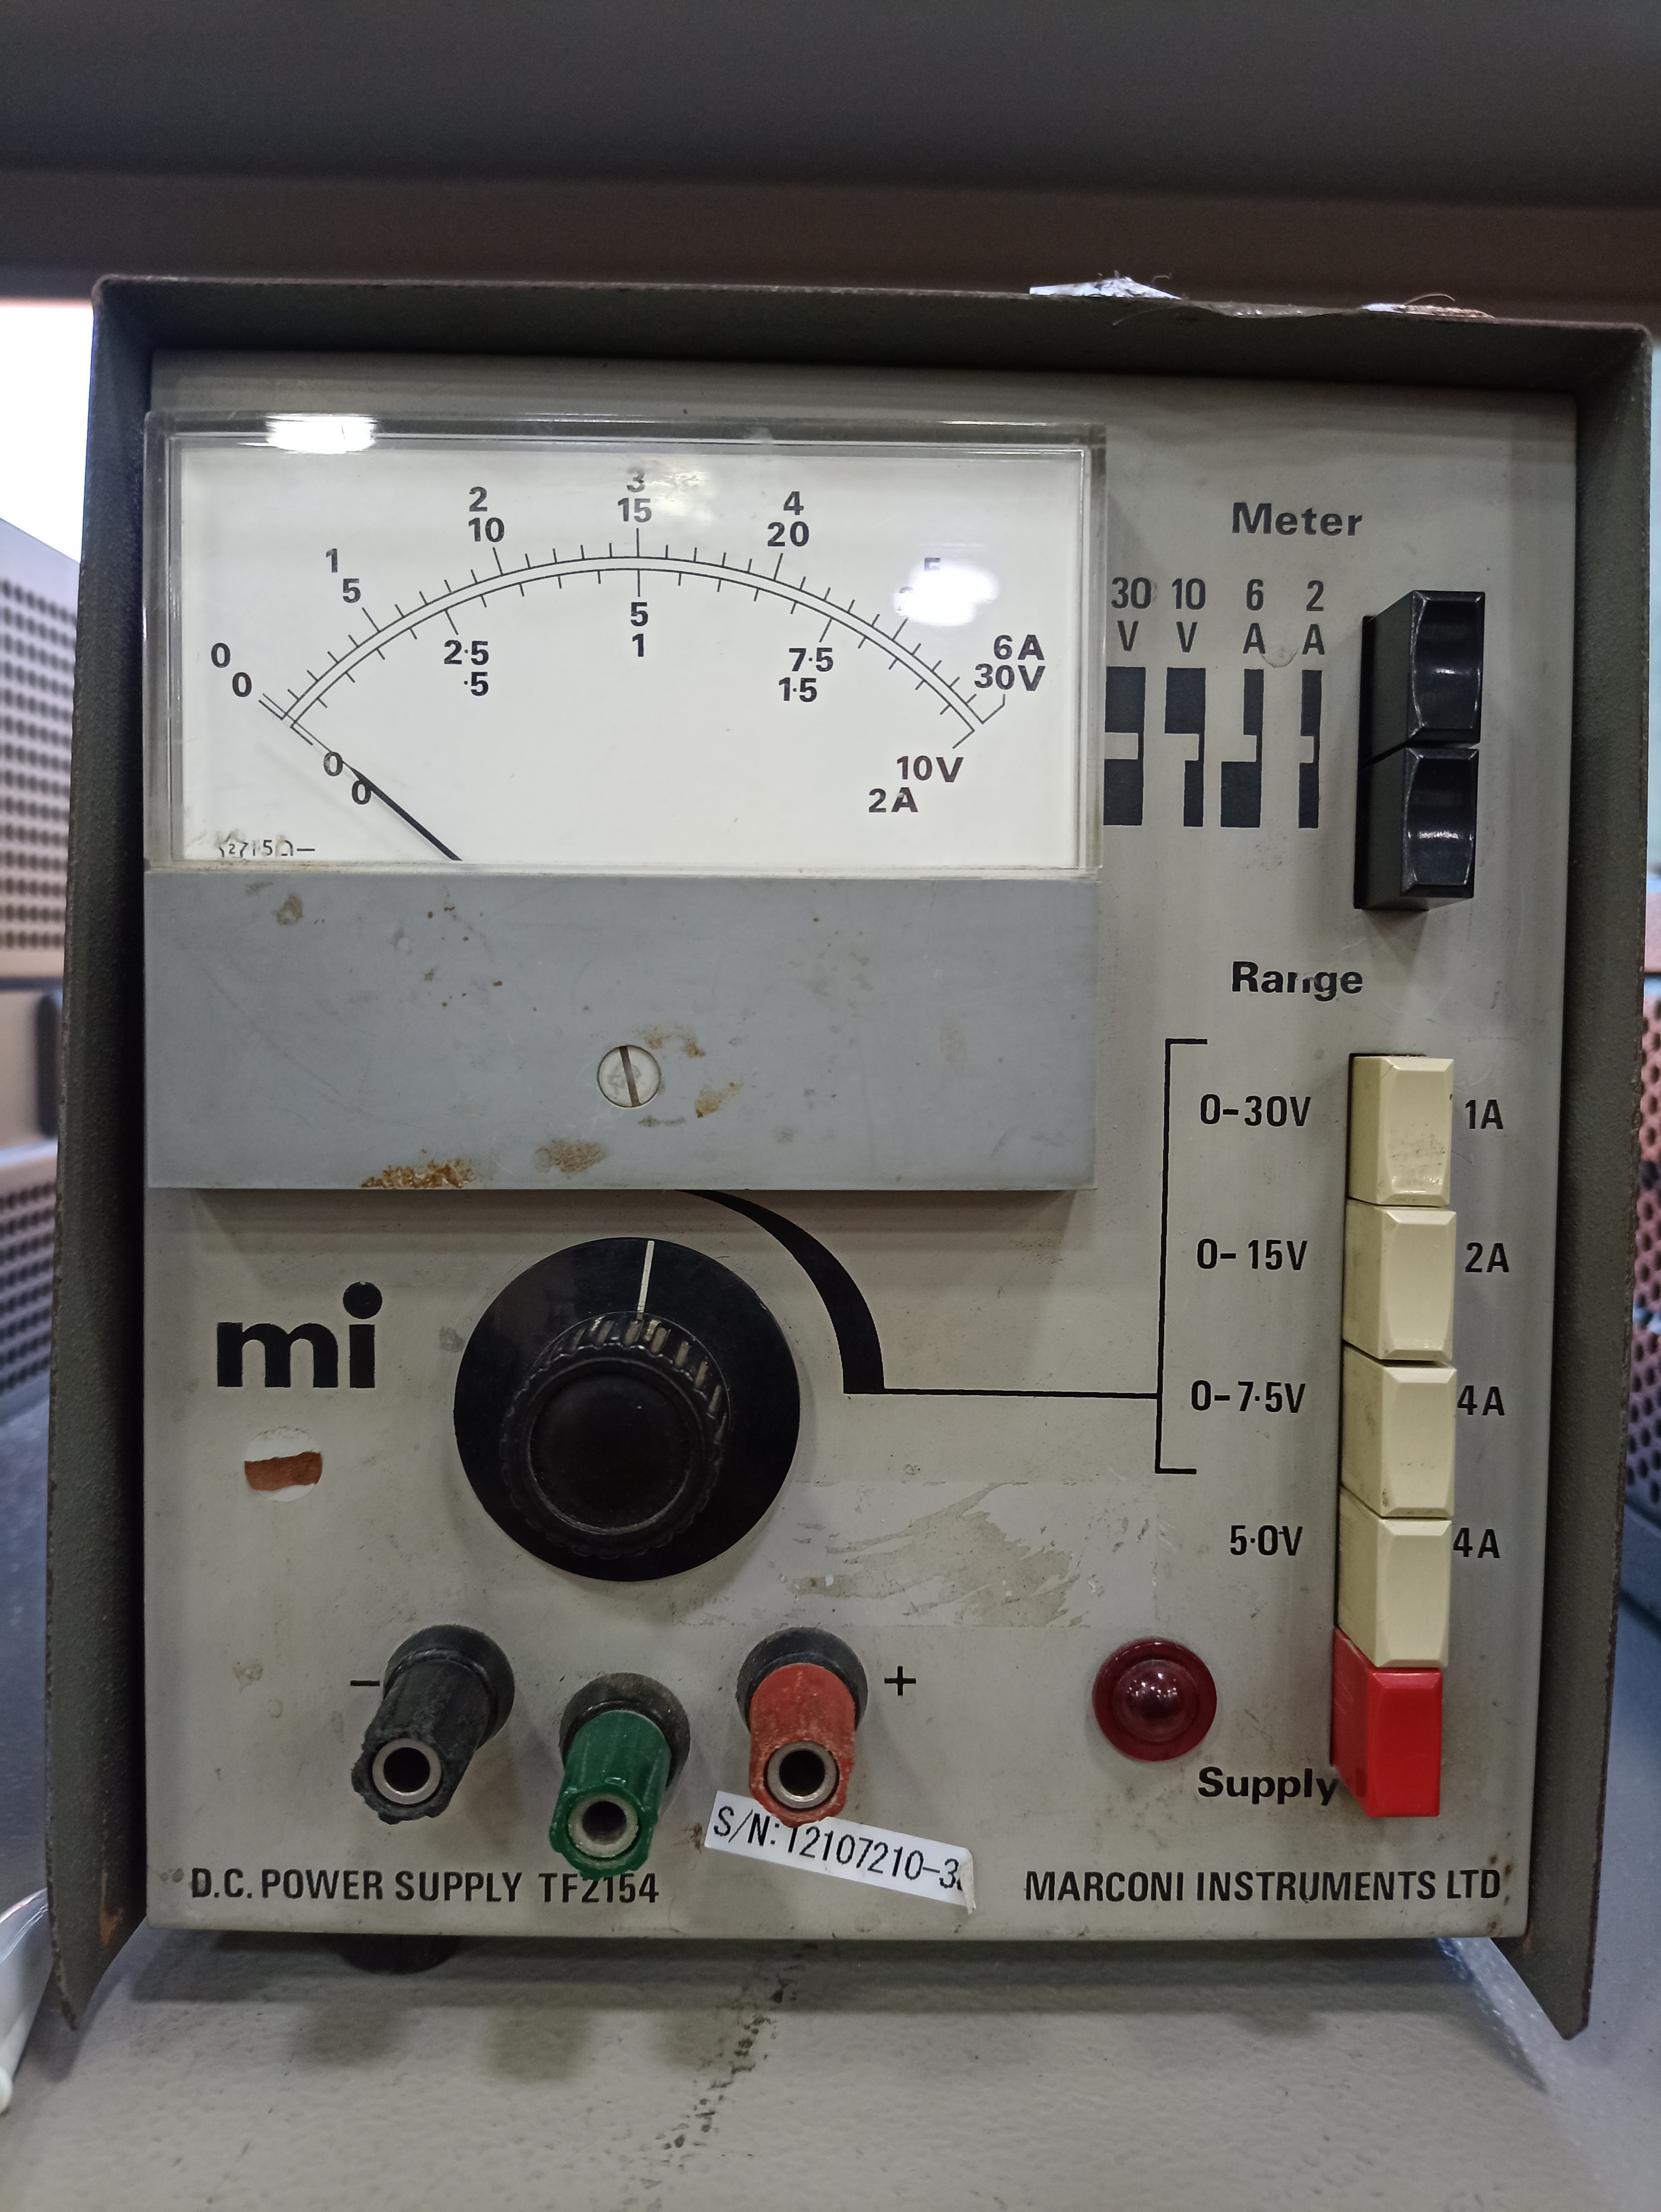
\includegraphics[width=0.6\textwidth]{images/mediciones_fuente.png}
    \caption{Fuente de alimentación utilizada.}
    \label{fig:mediciones_fuente}
\end{figure}


\subsubsection{FPGA}

La FPGA XXXXx generaba un pulso cuadrado. La misma puede observarse en la figura
\ref{fig:mediciones_fpga}.

La FPGA tenía la limitación de pasos de a 10\% para el duty.

\begin{figure}
  \centering
    \includegraphics[width=0.6\textwidth]{images/mediciones_fpga.png}
    \caption{Banco de medición}
    \label{fig:mediciones_fpga}
\end{figure}


\subsection{Mediciones realizadas}

Las mediciones consistieron en mediciones en del dominio del pulso de salida. Se
midieron tiempo de crecimiento, tiempo de decaimiento, amplitud máxima, y ancho
a medio máximo (\textit{FWHM} del inglés \textit{Full Width at Half Maximum}).

Se realizaron distintas mediciones para distintas condiciones del circuito. Se
barrió para el pulso digital de entrada, el ciclo de trabajo, y para la fuente
de alimentación distintos valores de tensión.

\begin{itemize}
    \item Para la amplitud de la fuente, se utilizaron valores de \qty{5}{\volt} y
        \qty{7}{\volt}.
        \begin{itemize}
            \item \qty{5}{\volt} por ser un valor fácilmente obtenible en los
                sistemas UWB de referencia.
            \item \qty{7}{\volt} por ser la máxima amplitud tolerable por el circuito.
                Tensiones de alimentación mayores a estas resultan en corrientes de
                polarización mayores a las máximas admisibles dado los
                dimensionamientos de las pistas de los PCBs.
        \end{itemize}
    \item El ciclo de trabajo se barrió entre \qty{50}{\percent} y
        \qty{70}{\percent}.
        \begin{itemize}
            \item Se tomo 50\% como límite inferior por ser un valor fácilmente
                obtenible como división de un reloj digital.
            \item Se tomo 70\% como límite superior ya que se observó que valores
                superiores a este resultaban en un pulso bipolar con amplitudes
                negativas decrecientes, y por lo tanto, amplitudes de pulso
                decrecientes.
            \item La teoría no indicaba un límite superior para el ciclo de
                trabajo. Sin embargo, este se observó en la práctica debido a no
                idealidades en el pulso de salida del driver, que no era
                perfectamente cuadrado.
        \end{itemize}
\end{itemize}

\begin{figure}
  \centering
    \includegraphics[width=0.6\textwidth]{images/banco_medicion.png}
    \caption{Banco de medición}
    \label{fig:banco_medicion}
\end{figure}

\subsection{Resultados}

En las figuras \ref{fig:mediciones_5v_50}, \ref{fig:mediciones_5v_70},
\ref{fig:mediciones_7v_50}, \ref{fig:mediciones_7v_60},
\ref{fig:mediciones_7v_70} pueden observarse los resultados en diversas capturas de pantalla
tomadas del osciloscopio.

Se observó en las mediciones una amplitud de pulso creciente con mayor ciclo de
trabajo y mayor amplitud de pulso, como era esperado. La menor amplitud de pulso
obtenida fue de \qty{380}{\milli\volt} para un $V_{cc}$ de \qty{5}{\volt} y un D
de \qty{50}{\percent}, y la mayor fue de \qty{1.12}{\volt} para un $V_{cc}$
de \qty{7}{\volt} y un D de \qty{70}{\percent}

En cuanto al ancho de pulso, se mantuvo aproximadamente constante en
\qty{160}{\pico\second}, al igual que los tiempos de crecimiento y
decrecimiento, que se mantuvieron constantes en \qty{90}{\pico\second}.

En la tabla \ref{tab:mediciones_resultados} pueden observarse los resultados obtenidos.

\begin{figure}
  \centering
    \includegraphics[width=0.6\textwidth]{images/mediciones/vcc_5v_duty_50.png}
    \caption{Salida @ $V_{cc}$ \qty{5}{\volt}, D \qty{50}{\percent} }
    \label{fig:mediciones_5v_50}
\end{figure}

\begin{figure}
  \centering
    \includegraphics[width=0.6\textwidth]{images/mediciones/vcc_5v_duty_70.png}
    \caption{Salida @ $V_{cc}$ \qty{5}{\volt}, D \qty{70}{\percent} }
    \label{fig:mediciones_5v_70}
\end{figure}

\begin{figure}
  \centering
    \includegraphics[width=0.6\textwidth]{images/mediciones/vcc_7v_duty_50.png}
    \caption{Salida @ $V_{cc}$ \qty{7}{\volt}, D \qty{50}{\percent} }
    \label{fig:mediciones_7v_50}
\end{figure}

\begin{figure}
  \centering
    \includegraphics[width=0.6\textwidth]{images/mediciones/vcc_7v_duty_60.png}
    \caption{Salida @ $V_{cc}$ \qty{7}{\volt}, D \qty{60}{\percent} }
    \label{fig:mediciones_7v_60}
\end{figure}

\begin{figure}
  \centering
    \includegraphics[width=0.6\textwidth]{images/mediciones/vcc_7v_duty_70.png}
    \caption{Salida @ $V_{cc}$ \qty{7}{\volt}, D \qty{70}{\percent} }
    \label{fig:mediciones_7v_70}
\end{figure}

\begin{table}
\centering
\begin{tabular}{ccccccc}
\hline
$V_{cc}$ [\unit{\volt}] & $D$ [\unit{\percent}] & $A$ [\unit{\volt}] &
    $FWHM$ [\unit{\pico\second}] & $\qty{3}{\dB} \ B$ [\unit{\giga\hertz}]& $t_r$
    [\unit{\pico\second}]& $t_f$ [\unit{\pico\second}]\\
\hline
5 & 50 & 0.380 & 159 & 7.5 & 93 & 88 \\
5 & 70 & 0.625 & 161 & 3.6 & 93 & 91 \\
7 & 50 & 0.702 & 162 & 3 & 93 & 93 \\
7 & 60 & 0.909 & 164 & 3 & 94 & 95 \\
7 & 70 & 1.120 & 165 & 3 & 95 & 96 \\
\hline
\end{tabular}
\caption{Resultados de mediciones.}
\label{tab:mediciones_resultados}
\end{table}

\subsubsection{Comparación contra simulación}

En las figuras pueden observarse los resultados de las mediciones obtenidas
superpuestos con los resultados de simulación para las mismas condiciones de
trabajo (amplitud de alimentación y ciclo de trabajo).

Para las simulaciones, se toman dos resultados: el de una simulación "ideal", 
indicada como "esquemático ideal" en las leyendas, que se corresponde a una simulación
sin contemplar parásitos de ningún tipo. El otro resultado corresponde a una simulación
mas completa, en las leyendas "Layout", es una simulación en la que se extrajeron
previamente los efectos parásitos del PCB, y se incorporaron en la simulación
del pulso.

Se realizan las comparaciones en el dominio del tiempo y de la frecuencia.

En el dominio del tiempo, se observa una buena coincidencia entre la amplitud
de los pulsos y el ancho. Se observa una diferencia en el \textit{ringing} de ambos.
Las simulaciones prácticamente no presentan oscilaciones alrededor del pulso,
mientras que las mediciones las presentan tanto previa como posteriormente.
También se observa un segundo pulso de menor amplitud siguiendo al primero.

Como causa de estas discrepancias, se descarta un efecto del PCB no modelado, 
ya que los parásitos de esta estructura fueron extraídos por una simulación 
electromagnética, y sus efectos contemplados en las simulaciones del \textit{layout}.

Estas  discrepancias sugieren una limitación en el modelado de alguno de los 
dispositivos, tanto el SRD como el Schottky. Las simulaciones predijeron correctamente
la amplitud y el ancho de los pulsos resultantes, pero fallaron en predecir 
el ringing y el pulso secundario.

\textcolor{red}{  
En el dominio de la frecuencia, se observa coincidencia entre los anchos de banda de los
pulsos.
EN REALIDAD NO, SE VE QUE EL PULSO 5V@50D TIENE UN ANCHO DE BANDA *MUCHO* MAYOR A 
LAS SIMULACIONES Y A LAS DEMÁS MEDICIONES.
HAY Q VER Q PASÓ AHÍ
}

\begin{figure}
  \centering
    \includegraphics[width=0.6\textwidth]{images/plots/Vcc_5V_duty_50_time_domain.png}
    \caption{Pulso @ $V_{cc}$ \qty{5}{\volt}, D \qty{50}{\percent} }
    \label{fig:plots_5v_50}
\end{figure}

\begin{figure}
  \centering
    \includegraphics[width=0.6\textwidth]{images/plots/Vcc_5V_duty_50_psd.png}
    \caption{PSD @ $V_{cc}$ \qty{5}{\volt}, D \qty{50}{\percent} }
    \label{fig:psd_5v_50}
\end{figure}

\begin{figure}
  \centering
    \includegraphics[width=0.6\textwidth]{images/plots/Vcc_5V_duty_70_time_domain.png}
    \caption{Pulso @ $V_{cc}$ \qty{5}{\volt}, D \qty{70}{\percent} }
    \label{fig:plots_5v_70}
\end{figure}

\begin{figure}
  \centering
    \includegraphics[width=0.6\textwidth]{images/plots/Vcc_5V_duty_70_psd.png}
    \caption{PSD @ $V_{cc}$ \qty{5}{\volt}, D \qty{70}{\percent} }
    \label{fig:psd_5v_70}
\end{figure}

\begin{figure}
  \centering
    \includegraphics[width=0.6\textwidth]{images/plots/Vcc_7V_duty_50_time_domain.png}
    \caption{Pulso @ $V_{cc}$ \qty{7}{\volt}, D \qty{50}{\percent} }
    \label{fig:plots_7v_50}
\end{figure}

\begin{figure}
  \centering
    \includegraphics[width=0.6\textwidth]{images/plots/Vcc_7V_duty_50_psd.png}
    \caption{PSD @ $V_{cc}$ \qty{7}{\volt}, D \qty{50}{\percent} }
    \label{fig:psd_7v_50}
\end{figure}

\begin{figure}
  \centering
    \includegraphics[width=0.6\textwidth]{images/plots/Vcc_7V_duty_60_time_domain.png}
    \caption{Pulso @ $V_{cc}$ \qty{7}{\volt}, D \qty{60}{\percent} }
    \label{fig:plots_7v_60}
\end{figure}

\begin{figure}
  \centering
    \includegraphics[width=0.6\textwidth]{images/plots/Vcc_7V_duty_60_psd.png}
    \caption{PSD @ $V_{cc}$ \qty{7}{\volt}, D \qty{60}{\percent} }
    \label{fig:psd_7v_60}
\end{figure}

\begin{figure}
  \centering
    \includegraphics[width=0.6\textwidth]{images/plots/Vcc_7V_duty_70_time_domain.png}
    \caption{Pulso @ $V_{cc}$ \qty{7}{\volt}, D \qty{70}{\percent} }
    \label{fig:plots_7v_70}
\end{figure}

\begin{figure}
  \centering
    \includegraphics[width=0.6\textwidth]{images/plots/Vcc_7V_duty_70_psd.png}
    \caption{PSD @ $V_{cc}$ \qty{7}{\volt}, D \qty{70}{\percent} }
    \label{fig:psd_7v_70}
\end{figure}

\subsection{Comparación con resultados de la literatura}
